%!TEX root=../document.tex

\section{First try}
Ich hab mich für das \textbf{Django REST Framework} entschieden, da ich schon mittelmäßige Erfahrung mit Django besitze und ich persönlich gerne mit Python arbeite. Es wurde auch Eve in Erwägung gezogen aber da ich schon mit Django gearbeitet habe, habe ich mich für diese Variante entschieden.

\subsection{Quickstart Tutorial}
\subsubsection{Projekt aufsetzen}
Der erste Schritt war es ein Django Projekt zu erstellen und alle nötigen Packages mit zu installieren.

\textbf{Virtual Environment erzeugen}
Zuerst wurde ein sogenanntes  \verb|Virtual Environment| erzeugt. Dieses erzeugt eine virtuelle Umgebung mit einer unabhängigen Installation von Python und allen anderen nötigen Zusatzpaketen.\\
Es gibt 2 Hauptgründe warum man ein Virtual Environment erzeugen sollte:
\begin{enumerate}
	\item Die Umgebung ist unabhängig vom System, d.h. es ist sichergestellt das jeder der das Projekt nun öffnet die gleichen Dependencies und Packages besitzt wie auf dem System auf dem das Projekt erstellt wurde
	\item Die lokale Installation auf dem System kann nicht verändert, beschädigt oder gelöscht werden
\end{enumerate}

Um die Umgebung aufzusetzen und diese zu verwenden, werden folgende Kommandos verwendet:

\begin{lstlisting}[language=bash]
virtualenv env
env\Scripts\activate
\end{lstlisting}

Nun werden alle packages welche installiert werden, in dieser virtuellen Umgebung installiert und sind somit isoliert.

\textbf{Packages installieren}
Die 2 nötigen Packages für das Beispiel sind \verb|django| und \verb|djangorestframework|, diese würden über pip installiert mit:

\begin{lstlisting}[language=bash]
pip install django
pip install djangorestframework
\end{lstlisting}

\textbf{Django Projekt erstellen}
Das tatsächliche Projekt wird über das \verb|django-admin.py| erstellt:

\begin{lstlisting}[language=bash]
django-admin.py startproject application .
cd tutorial
django-admin.py startapp quickstart
\end{lstlisting}

Nun wird noch die Datenbank synchronisiert:

\begin{lstlisting}[language=bash]
manage migrate
\end{lstlisting}

\textbf{Admin-User erstellen}
Um die Datenbank zu verwalten wird ein \verb|super user| benötigt. Dieser kann auch mit \verb|manage.py| erstellt werden:

\begin{lstlisting}[language=bash]
manage createsuperuser
\end{lstlisting}

Nach dem Betätigen der Enter-Taste wird veranlasst einen Namen, eine E-Mail Adresse und ein Passwort anzugeben. Für das Beispiel wurde \textbf{admin} mit dem Passwort \textbf{schueler} gewählt.

\subsubsection{Serializer definieren}
Es wird im Verzeichnis \verb|application/quickstart| ein File namens \verb|serializers.py| erstellt.

In diesem File wird eine \verb|UserSerializer| Klasse erstellt, welche von \\ \verb|serializers.HyperlinkedModelSerializer| erbt. Dies beschreibt einfach nur wie die Relationen zueinander stehen, es können auch klassisch Primary Key und andere Beziehungen verwendet werden, aber HyperLinked Beziehungen sind gutes \textbf{REST}ful design.

In dieser Klasse wird beschrieben welche Felder der User besitzt, d.h. wenn ein neuer User erstellt welche Felder alle ausgefüllt werden müssen. Es wurden folgende Attribute entschieden:

\begin{itemize}
	\item URL (Wird automatisch erstellt)
	\item Vorname
	\item Nachname
	\item E-Mail
	\item Passwort (Fungiert derweil nicht als richtiges Passwort, nur als Feld angelegt)
\end{itemize}

\begin{lstlisting}[language=python]
class UserSerializer(serializers.HyperlinkedModelSerializer):
	class Meta:
		model = User
		fields = ('url', 'first_name', 'last_name', 'email', 'password')
\end{lstlisting}

\subsubsection{View definieren}
Im Verzeichnis \verb|application/quickstart| wird das File \verb|views.py| geöffnet. In diesem wird die Klasse \verb|UserViewSet| erstellt. Diese Klasse definiert wie die Query für die User ausschaut, wenn diese angezeigt werden sollen. In dem Beispiel schaut die Query folgendermaßen aus:\\
\verb|User.objects.all().order_by('-date_joined')|. Zusätzlich wird noch der Serializer angegeben:

\begin{lstlisting}[language=Python]
class UserViewSet(viewsets.ModelViewSet):
	queryset = User.objects.all().order_by('-date_joined')
	serializer_class = UserSerializer
\end{lstlisting}

\subsubsection{URLs definieren}
Der nächste Schritt besteht darin die nötigen URLs zu definieren.

Da in dem Beispiel nicht einzelen Views verwendet werden sondern \verb|ViewSet|s, kann ein \verb|Router| verwendet werden für die URLs. Praktisch funktioniert es so, dass zuerst ein router definiert wird, in diesem Router dann das ViewSet der User \textbf{registriert} wird, und dieser Router anschließend als URL \textbf{included} wird. 

Zusätzlich werden noch URLs vom \verb|rest_framework| definiert um Login- und LogoutViews anzuzeigen: 

\begin{lstlisting}[language=python]
router = routers.DefaultRouter()
router.register(r'users', views.UserViewSet)

urlpatterns = [
url(r'^', include(router.urls)),
url(r'^api-auth/', include('rest_framework.urls', namespace='rest_framework'))
]
\end{lstlisting} 

\subsubsection{Einstellungen anpassen}
Bevor man die ersten Ergebnisse sehen kann, müssen im File \verb|settings.py| noch einige Einstellungen angepasst werden.

Der erste Schritt ist es in der \verb|INSTALLED_APPS| Liste unser Framework hinzuzufügen:

\begin{lstlisting}[language=Python]
INSTALLED_APPS = [
	'django.contrib.admin',
	'django.contrib.auth',
	'django.contrib.contenttypes',
	'django.contrib.sessions',
	'django.contrib.messages',
	'django.contrib.staticfiles',
	'rest_framework'
	]
	
\end{lstlisting}

Zusätzlich wird noch eine Einschränkung hinzugefügt, dass nur der Admin User alles anzeigen lassen kann und es wird noch eine Seitennummerierung eingefügt:

\begin{lstlisting}[language=Python]
REST_FRAMEWORK = {
	'DEFAULT_PERMISSION_CLASSES': [
	'rest_framework.permissions.IsAdminUser',
	],
	'PAGE_SIZE': 10
	}
\end{lstlisting}

\subsubsection{Beispiel testen}
\textbf{Webservice starten}

Der webservice muss zuerst in der Konsole gestartet werden
\begin{lstlisting}[language=Bash]
manage runserver
\end{lstlisting}

\textbf{Zugriff durch Browser}
Es kann nun auf den service via Browser zugegriffen werden über die Adresse \verb|localhost:8000|.

Im Root Verzeichnis bekommt man lediglich eine JSON Response mit folgendem Inhalt:

\begin{lstlisting}[language=JSON]
HTTP 403 Forbidden
Allow: GET, HEAD, OPTIONS
Content-Type: application/json
Vary: Accept

{
	"detail": "Authentication credentials were not provided."
}
\end{lstlisting}

\textbf{Login als Admin}
Um die User sehen zu können muss sich zuerst einloggen als Admin:

\begin{minipage}{\linewidth}
	\centering
	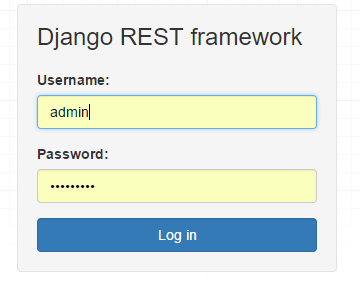
\includegraphics[width=0.5\linewidth]{images/login}
	\figcaption{Login als Admin}
\end{minipage}

Nun erhält man folgende Antwort:

\begin{lstlisting}[language=JSON]
HTTP 200 OK
Allow: GET, HEAD, OPTIONS
Content-Type: application/json
Vary: Accept

{
	"users": "http://localhost:8000/users/"
}
\end{lstlisting}


\textbf{User einsehen und hinzufügen}

Um nun die CRUD-Funktionalität nutzen zu können muss auf die URL \verb|http://localhost:8000/users| gewechselt werden.

Man kann nun alle User einsehen oder neue hinzufügen:

\begin{minipage}{\linewidth}
	\centering
	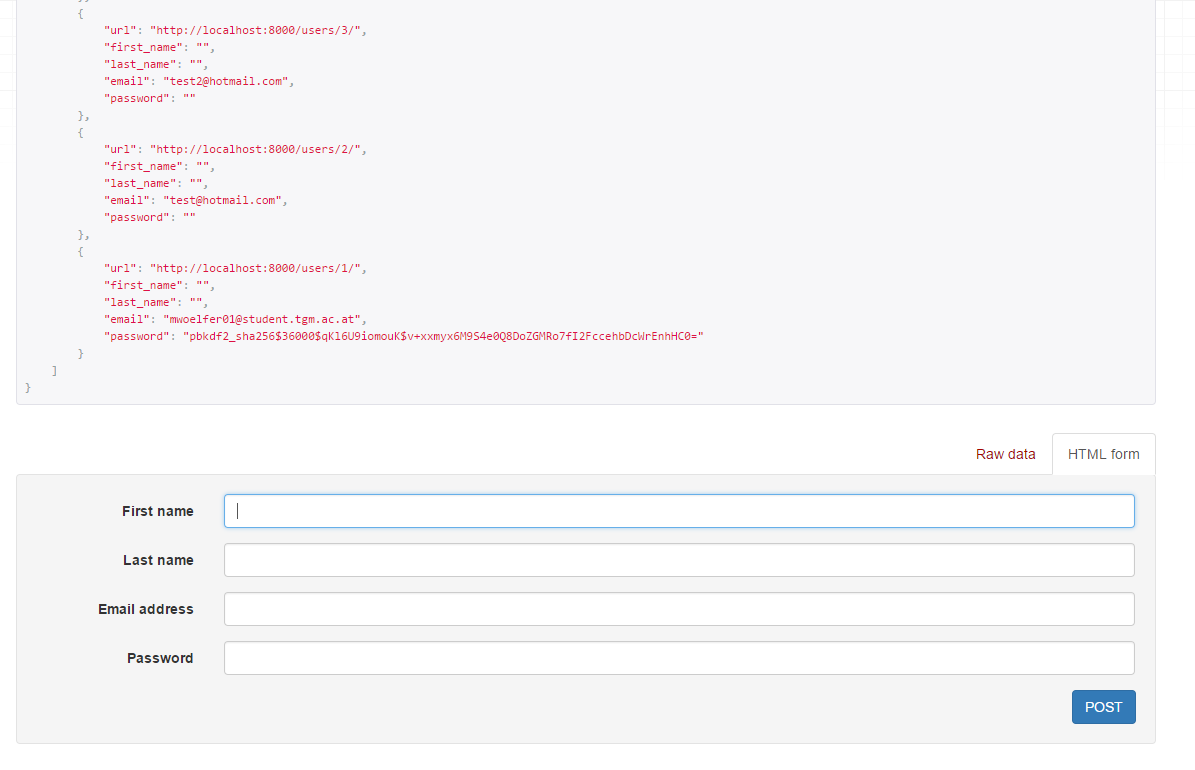
\includegraphics[width=1\linewidth]{images/read_add}
	\figcaption{User einsehen oder hinzufügen}
\end{minipage}

\clearpage
\textbf{User verändern oder löschen}
Da jeder User eine eigene URL besitzt, kann man diese auch einzeln einsehen und anschließend verändern bzw. löschen:

\begin{minipage}{\linewidth}
	\centering
	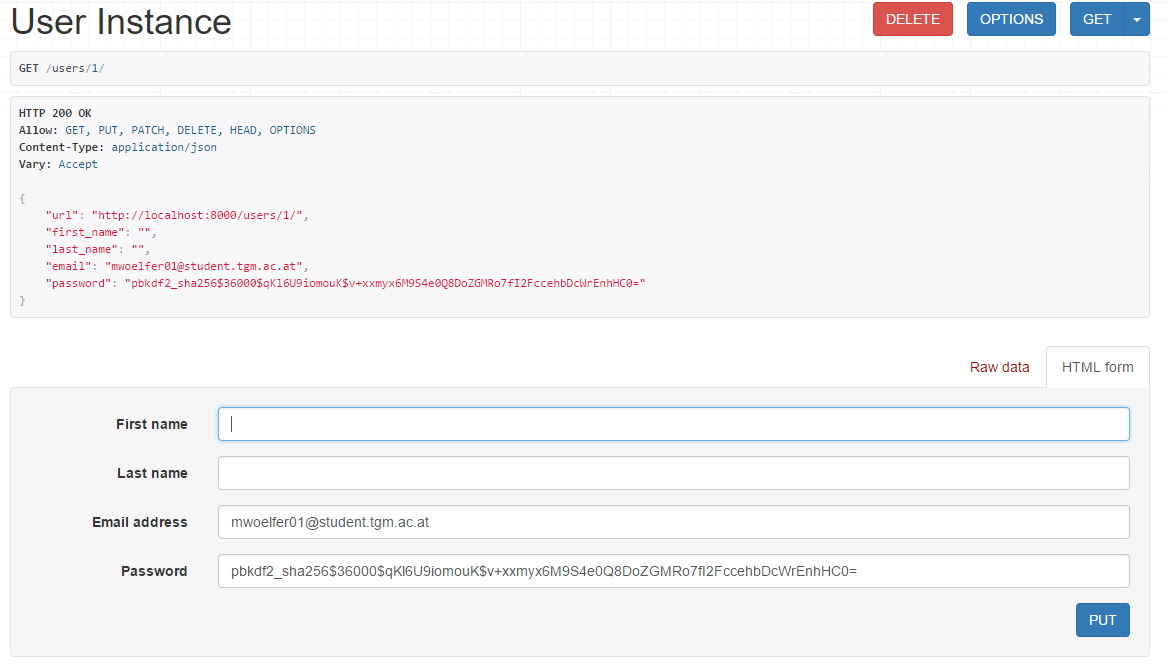
\includegraphics[width=1\linewidth]{images/change_delete}
	\figcaption{User kann verändert oder gelöscht werden}
\end{minipage}

\subsection{Tutorial mit User Authentifizierung}
Nun das die Grundlagen verstanden wurden durch das Quickstart Tutorial, kann ein Projekt erstellt werden welches genau in die Thematik eintaucht. Auf der Django-REST Framework Seite gibt es ein Tutorial welchein verschiedene Abschnitte unterteilt ist, welches nun Schritt für Schritt abgearbeitet und verstanden wird. 

\subsubsection{Projekt erstellen}
\textbf{Virtuelle Umgebung}

Da schon für das erste Tutorial eine virtuelle Umgebung erstellt wurde, muss keine neue definiert werden aber es muss ein Paket hinzugefügt werden:

\begin{lstlisting}[language=bash]
pip install pygments
\end{lstlisting}

Dieses Paket dient für Code-Highlighting

\textbf{Django Projekt erstellen}

Wie bereits gewohnt wird das Projekt erstellt mit: 

\begin{lstlisting}[language=bash]
django-admin startproject application_authentication
\end{lstlisting}

\textbf{App erstellen}

Wie auch im ersten Tutorial wird nun eine App erstellt:

\begin{lstlisting}[language=bash]
manage startapp snippets
\end{lstlisting}

Diese muss natürlich in \verb|application_authentication/settings.py|, sowie das \verb|rest_framework|, zu den \verb|INSTALLED_APPS| hinzugefügt werden:

\begin{lstlisting}[language=python]
INSTALLED_APPS = (
...
'rest_framework',
'snippets.apps.SnippetsConfig',
)
\end{lstlisting}

\section{Second try}
Da der erste Versuch nicht funktionierte, wurde auf eine Realisierung in JavaEE gesetzt mit Unterstützung von \verb|Spring Boot|, \verb|Spring Security|, \verb|Spring Data JPA| und der Datenbank \verb|HSQL|. Es wurde mit folgendem Tutorial gearbeitet:

\href{https://hellokoding.com/registration-and-login-example-with-spring-security-spring-boot-spring-data-jpa-hsql-jsp/}{https://hellokoding.com/registration-and-login-example-with-spring-security-spring-boot-spring-data-jpa-hsql-jsp/}
 
Das Endergebnis ist ein RESTful Webservice bei welchem man sich einloggen und registrieren kann und mit einer Willkommensnachricht begrüßt wird. 

\subsection{Dependencies definieren}
Die dependencies, d.h. welche Framework verwendet wird. Normalerweise würde das bedeuten die jeweiligen \verb|.jar| Files herunterzuladen und dem Build-Path hinzuzufügen, aber dank Maven kann man dies ganz einfach im \verb|pom.xml| File definieren:

\begin{lstlisting}[language=xml]
<dependencies>

	<dependency>
		<groupId>org.springframework.boot</groupId>
		<artifactId>spring-boot-starter-web</artifactId>
	</dependency>
  
	<dependency>
		<groupId>org.springframework.boot</groupId>
		<artifactId>spring-boot-starter-data-jpa</artifactId>
	</dependency>
  
	<dependency>
		<groupId>org.springframework.boot</groupId>
		<artifactId>spring-boot-starter-security</artifactId>
	</dependency>
  
	<dependency>
		<groupId>org.hsqldb</groupId>
		<artifactId>hsqldb</artifactId>
		<scope>runtime</scope>
	</dependency>
  
  
	<dependency>
		<groupId>org.springframework.boot</groupId>
		<artifactId>spring-boot-starter-tomcat</artifactId>
		<scope>provided</scope>
	</dependency>
  
	<dependency>
		<groupId>org.springframework.boot</groupId>
		<artifactId>spring-boot-starter-test</artifactId>
		<scope>test</scope>
	</dependency>
  
	<dependency>
		<groupId>org.apache.tomcat.embed</groupId>
		<artifactId>tomcat-embed-jasper</artifactId>
		<scope>provided</scope>
	</dependency>
  
	<dependency>
		<groupId>javax.servlet</groupId>
		<artifactId>jstl</artifactId>
	</dependency>
  
	<dependency>
		<groupId>junit</groupId>
		<artifactId>junit</artifactId>
	</dependency>
  
</dependencies>
\end{lstlisting}

Zusätzlich wird noch das \verb|springframework| plugin defniert:

\begin{lstlisting}[language=xml]
<build>
	<plugins>
		<plugin>
			<groupId>org.springframework.boot</groupId>
			<artifactId>spring-boot-maven-plugin</artifactId>
		</plugin>
	</plugins>
</build>
\end{lstlisting}

\subsection{Entities definieren}
Mit \verb|hsql| wird eine table durch die annotation \verb|@Entitity| definiert. Es wird eine Klasse User erstellt, welche folgende Attribute besitzt:

\begin{itemize}
	\item Long id
	\item String username
	\item String password
	\item String passwordConfirm
	\item Set<Role> roles
\end{itemize} 

Danach werden Getter- und Settermethoden definiert. Zu beachten ist, dass id den eindeutigen Primary Key repräsentiert und somit bei \verb|getId()| die Annotations \verb|@Id| und \verb|@GenerateValue(strategy = Generationtype.AUTO)| benötigt werden.

\begin{lstlisting}[language=java]
package com.hellokoding.auth.model;

import javax.persistence.*;
import java.util.Set;

@Entity
@Table(name = "user")
public class User {
	private Long id;
	private String username;
	private String password;
	private String passwordConfirm;
	private Set<Role> roles;
	
	@Id
	@GeneratedValue(strategy = GenerationType.AUTO)
	public Long getId() {
		return id;
	}
	
	public void setId(Long id) {
		this.id = id;
	}
	
	public String getUsername() {
		return username;
	}
	
	public void setUsername(String username) {
		this.username = username;
	}
	
	public String getPassword() {
		return password;
	}
	
	public void setPassword(String password) {
		this.password = password;
	}
	
	@Transient
	public String getPasswordConfirm() {
		return passwordConfirm;
	}
	
	public void setPasswordConfirm(String passwordConfirm) {
		this.passwordConfirm = passwordConfirm;
	}
	
	@ManyToMany
	@JoinTable(name = "user_role", joinColumns = @JoinColumn(name = "user_id"), inverseJoinColumns = @JoinColumn(name = "role_id"))
	public Set<Role> getRoles() {
		return roles;
	}
	
	public void setRoles(Set<Role> roles) {
		this.roles = roles;
	}
}
\end{lstlisting}